%
% Gaze Tracking in Semi-Autonomous Grasping
% JEMR special issue on ECEM2007 abstracts
% Castellini
%

% ------------------------------------------------- for reviewer 1:
% . your doubts about Tc are surprising, since I had a whole
%   subsection about that. I am thinking I might have got the
%   submission wrong! anyway, now the subsection is back, also with
%   references to signals theory, which should - I hope - fix the problem.
% . 47Hz - I admit that has no justification. I have added a few lines of
%   explanation.
% . Fig. 5 has been improved by writing numbers in the caption
% . typoes fixed
%
% ------------------------------------------------- for reviewer 2:
% . your concerns about fixation vs. raw data are absolutely correct.
%   I have amended and clarified this in Section ``experimental setup''.
% . your remark that experiments are short is indeed correct, but one of the
%   very points of the experiment itself was to determine how much data
%   was required at least to get good models... in other words: for my
%   purpose, the shorter, the better.
% . more about SVMs, Tc and C has been put in.
% . typoes corrected.
%
% ------------------------------------------------- for reviewer 3:
% . some of the questions under your point (1) cannot be
%   answered now - the setup is no longer in place and data have then
%   been collected at 47Hz since this was the streaming frequency of
%   the gaze tracker. more on the setup, including a figure of the
%   stimulus, has been added in the section called ``building the data
%   set''. I hope this will fix, at least, some of your concerns.
% . I have explained in a somehow deeper detail the grid search for
%   the SVM hyperparameters.
% . references, typoes and bibliography have been fixed.
%

\documentclass[jou,a4paper,notxfonts]{apa}
\usepackage{graphicx} 
\usepackage{palatino}
\usepackage{float}
\usepackage{url}
\usepackage{amsmath}
\usepackage[psamsfonts]{amssymb}

\def\RR{\mathbb{R}}
\def\NN{\mathbb{N}}
\def\xx{\mathbf{x}}
\def\yy{\mathbf{y}}
\def\ww{\mathbf{w}}
\def\aa{\boldsymbol{\alpha}}
\def\bb{\boldsymbol{\beta}}
\def\ee{\mathbf{e}}
\def\dd{\mathbf{d}}
\def\mdd{\tilde{\dd}}
\def\b{\mathcal{B}}
\def\d{\mathcal{D}}

%%%%%%%%%%%%%%%%%%%%%%%%%%%%%%%%%%%%%%%%%%%%%%%%%%%%%%%%%%%%%%%%%%%%%%%%%%%%%%%%

\title{Gaze Tracking in Semi-Autonomous Grasping}

\author{Claudio Castellini}
\affiliation{LIRA-Lab, University of Genova, Italy}
\journal{Journal Of Eye Movement Research}
\volume{2(4):2,1-7}

\abstract{
  In critical human/robotic interactions such as, e.g., teleoperation
  by a disabled master or with insufficient bandwidth, it is highly
  desirable to have \emph{semi-autonomous} robotic artifacts interact
  with a human being. Semi-autonomous grasping, for instance, consists
  of having a smart slave able to guess the master's intentions and
  initiating a grasping sequence whenever the master wants to grasp an
  object in the slave's workspace.
  In this paper we investigate the possibility of building such an
  intelligent robotic artifact by training a machine learning system
  on data gathered from several human subjects while trying to grasp
  objects in a teleoperation setup. In particular, we investigate the
  usefulness of gaze tracking in such a scenario. The resulting system
  must be light enough to be usable on-line and flexible enough to
  adapt to different masters, e.g., elderly and/or slow.
  The outcome of the experiment is that such a system, based upon
  Support Vector Machines, meets all the requirements, being $(a)$
  highly accurate, $(b)$ compact and fast, and $(c)$ largely
  unaffected by the subjects' diversity. It is also clearly shown that
  gaze tracking significantly improves both the accuracy and
  compactness of the obtained models, if compared with the use of the
  hand position alone. The system can be trained with something like
  $3.5$ minutes of human data in the worst case.
  \linebreak
  \linebreak
  {\bf Keywords: machine learning, gaze tracking, teleoperation}
}

\acknowledgements{The work is supported by the EU-funded project
NEURObotics (FP6-IST-001917). We thank Giulio Sandini and Giorgio
Metta of the Italian Institute of Technology and Francesco Orabona of
IDIAP for their support and suggestions.}
\shorttitle{Gaze in Semi-Autonomous Grasping}
\rightheader{Journal of Eye Movement Research, 2(4):2,1-7}
\leftheader{Claudio Castellini}

\begin{document}

\maketitle

%%%%%%%%%%%%%%%%%%%%%%%%%%%%%%%%%%%%%%%%%%%%%%%%%%%%%%%%%%%%%%%%%%%%%%%%%%%%%%%%
\section{Introduction}

\label{sec:intro}

Semi-autonomous teleoperation consists of having a robotic setup (the
\emph{slave}) work in a remote environment, guided by a human user
(the \emph{master}). In a basic setting, the cooperation between
master and slave is realised in such a way that the actions performed
by the master can be precisely and timely replicated by the slave. In
order to convey a feeling of telepresence, in particular, a high
bandwidth is required for the slave-to-master sensorial feedback
\cite{telesensation}. But, when any of the above conditions fails,
teleoperation must be somehow augmented. The slave could consist of a
set of surgical tools \cite{okamura} not immediately related to the
human fingers; or, the master could be a disabled person; or, lastly,
the master/slave communication bandwidth could be insufficient for a
timely and accurate transmission of sensorial feedback.

One of the possibilities to overcome these problems is that of making
the slave more intelligent by building into it \emph{internal models}
of the required actions \cite{kawato-99}. It is envisioned, in this
scenario, that the master should first train the slave to perform the
actions required, in a safe and controlled environment; and that this
acquired knowledge should then be used by the slave in real
situations, whenever the environment or the master's abilities do not
allow direct control. Upon detecting the master's intention to, e.g.,
grasp an object in its own workspace, the slave should take control
over, initiate and complete a grasping action possibly modelled upon
the user's style, and then return the control to the master. This is
what we call \emph{semi-autonomous grasping}.

As a minimum set of requirements, such a model should be
\emph{accurate} (it should be able to tell exactly when to start an
autonomous grasp, avoiding doing it when not required), \emph{fast},
since it must be used in real-time, and \emph{flexible}: it must adapt
well to different subjects' parameters (speed of reach, direction of
motion), abilities and intentions, and it must be trained in a
reasonably short amount of time.

In this paper we investigate the possibility of building such an
internal model, employing a machine learning system based upon a
Support Vector Machine (SVM) \cite{BGV92}. In \cite{clea07}, we
already showed some promising results related to the problem; here we
refine the data analysis and show the results of an experiment in
which seven subjects, of different ages and with slightly different
movement and gaze abilities, were placed in a real teleoperation
scenario; by repeatedly performing a fake grasping action, the
subjects would teach a SVM to recognise when they wanted to grasp an
object in the slave setup; this was achieved by simply fixating the
object, reaching for it and closing their hand. Here we carry the data
analysis to the end.

Data was gathered from the subjects using a magnetic tracker for the
position of the hand, and a gaze tracker in order to understand
whether the subject was fixating a particular object. One interesting
question is whether gaze tracking couldactually improve the situation.
The outcome of the experiment is that such a model can actually be
built, and that it fulfills all the requirements enumerated above: it
is highly accurate; the solution achieved is extremely compact; and
these characteristics are largely independent of the subjects'
abilities. The training phase is accomplished using about $3.5$
minutes of data gathered in real-time from each subject, in the worst
case. Lastly, the use of gaze tracking significantly improves the
obtained models, both as far as their accuracy and size is concerned.

The paper is structured as follows: we first describe the materials
and methods used in the experiment; we then go on to show the
experimental results, and lastly we draw conclusions and outline
future work.

%%%%%%%%%%%%%%%%%%%%%%%%%%%%%%%%%%%%%%%%%%%%%%%%%%%%%%%%%%%%%%%%%%%%%%%%%%%%%%%%
\section{Materials and Methods}

\label{sec:matmet}

\subsection{Subjects}

Seven subjects, four women and three men, aged $30$ to $73$,
volunteered to join the experiment. They were all right-handed and
fully able-bodied, and were given no knowledge of the aim of the
experiment. Four of the subjects were slightly visually
impaired.

\subsection{Setup and devices}

The subjects were asked to sit confortably in front of a clean
workspace, and a flat $17$ inches color monitor was placed in front of
them at a distance of about half a meter. They wore an Immersion
\emph{CyberGlove} data glove \cite{cyberglove} on their right hand,
and an Ascension \emph{Flock-of-Birds} (FoB) \cite{fob} sensor was
firmly mounted on top of their wrist. Lastly, an ASL \emph{E504} gaze
tracker \cite{e504} was placed on the left hand side of the
monitor. Figure \ref{fig:devices} shows the devices and setup.

\begin{figure*}[ht]
  \centering
    \begin{tabular}{cccc}
      \includegraphics[width=0.24\linewidth]{figs/glove.eps} &
      \includegraphics[width=0.24\linewidth]{figs/e504.eps} &
      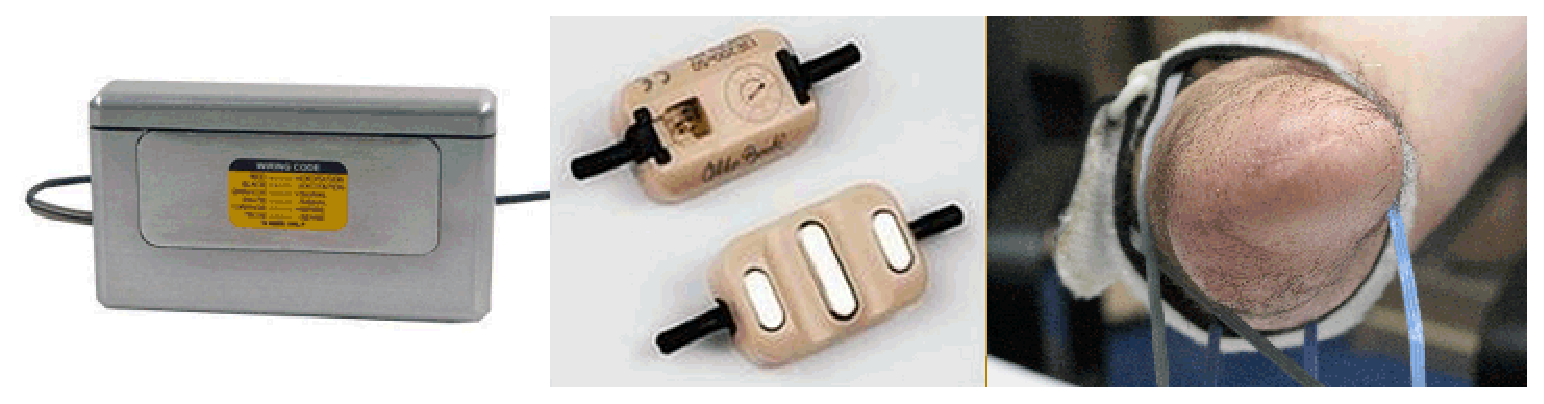
\includegraphics[width=0.24\linewidth]{figs/setup.eps} &
      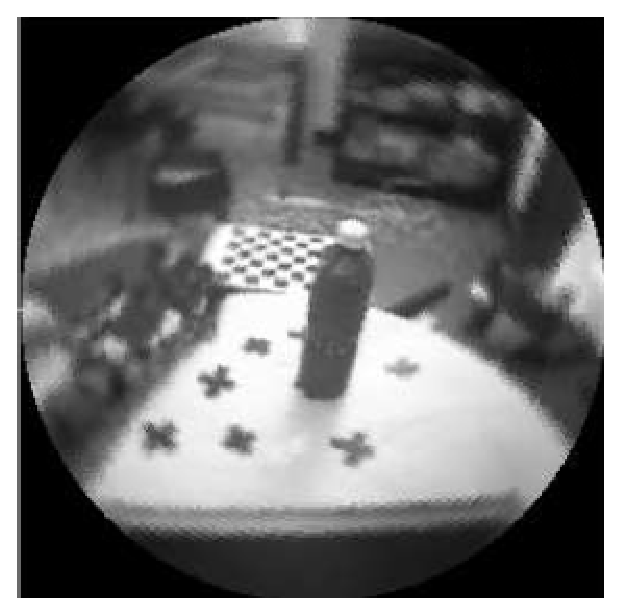
\includegraphics[height=0.18\linewidth]{figs/stimulus.eps} \\
      $(a)$ & $(b)$ & $(c)$ & $(d)$ \\
    \end{tabular}
    \caption{The devices and setup used for the experiment, and
    the stimulus presented to the human subjects: $(a)$ the
    Immersion CyberGlove with the Flock-of-Birds sensor just above the
    wrist; $(b)$ the ASL E504 gaze tracker (pan/tilt near-infrared
    camera); $(c)$ the whole setup; $(d)$ a black-and-white image
    of the stimulus, that is, an example of what a subject might
    see in the monitor.}
    \label{fig:devices}
\end{figure*}

The FoB had the $X/Y$ plane parallel to the workspace horizontal
plane. The device returns $6$ double-precision numbers describing the
position ($x$, $y$ and $z$ in inches) and rotation (azimuth, elevation
and roll in degrees) of the sensor with respect to a magnetic basis
mounted about one meter away from the subject.  The spatial resolution
of the acquired data is $0.1$ inches and $0.5$ degrees.

The E504, after the standard calibration phase, returns one true/false
value, denoting validity of the gaze coordinates (that is, the pupil
being in sight of the camera and correctly recognised), and two
double-precision numbers indicating the coordinates of the subject's
gaze with respect to the monitor. Its precision is about $1$ degree
which, we verified, corresponded to less than one pixel precision on
the monitor, which was considered acceptable. The device can nominally
stream at up to $50$Hz. We configured it in order not to filter in any
way the gaze signal, so that we could read the ``raw'' pupil movement;
notice that, however, the signal was actually filtered off-line, later
on, during the data analysis, as described below.

The CyberGlove was used as an on-off switch, to detect when the
subject's hand would close, by monitoring one of its sensors via a
threshold.

The monitor showed the slave's workspace; the slave is the humanoid
platform Babybot, composed of two colour cameras, a commercial
$6$-degrees-of-freedom robotic arm, a pan/tilt head and a humanoid
hand (see, e.g., \cite{babybotHum2005}). During the experiment, we
only employed one of its colour cameras. Figure \ref{fig:devices},
panel $(d)$ (reproduced from \cite{babybotHum2005}), shows a
black-and-white representation of the workspace as seen on the monitor
by the subject, that is, the ``stimulus'' presented to those who
joined the experiment.

All data were collected, synchronised, and saved in real time at a
frequency of slightly less than $50$Hz, this being the best frequency
obtained from the gaze tracker.

\subsection{Method}

The subjects were asked to initially keep their right hand and arm in
a resting position. The monitor showed the slave's workspace, in which
several objects could be clearly seen, and a moving red cross
corresponding to the detected subject's gaze. The subjects were then
instructed, upon a request by the experimenter, to look at one of the
objects on the monitor and then to move their hand as if to reach and
grasp it, signalling the act of grasping by closing their right
hand. The red cross on the screen turned green when the hand was
closed, to confirm the grasping.

This fake grasping act was repeated for $15$ to $21$ times, each time
with a different object (therefore, toward a different position) seen
on the monitor. The maximum duration of the whole experiment for a
single subject was about $3.5$ minutes, resulting in no tiredness.

\subsection{Building the data set}
\label{subsec:dataset}

The first question was \emph{what} pieces of data to consider to train
our machine, that is, how to filter and/or manipulate the data
obtained from the setup. It is well-known that, when a human subject
wants to grasp an object, he/she fixates the desired object and then
performs the reaching action, without looking at his own hand while
reaching (see, e.g., \cite{johansson01}). Therefore, we considered
$(a)$ the average of the subjects' hand velocity, $(b)$ the variance
of the subjects' gaze coordinates and $(c)$ the information whether
the subjects' right hand was open or closed. We then expect, while
fixating and reaching,

\begin{enumerate}

  \item the gaze coordinates to hover around the point on the screen
    where the desired object is seen; that is, their standard
    deviation over some time to be \emph{small}; and

  \item the hand to move towards the object on the screen, that is,
    the hand velocity components to be on average \emph{large}.

\end{enumerate}

The instants in which the hand is closed signal the intention to
grasp, whereas those when the hand is open represent negative
examples. Data $(a)$ were easily obtained by differentiating in time
the hand position $x,y,z$ coordinates obtained from the FoB and then
averaging these numbers over a certain time window (see below); data
$(b)$ were obtained by evaluating the standard deviation over the same
time window of the gaze coordinates obtained from the E504; and lastly
data $(c)$ was obtained directly from the CyberGlove. (The samples
corresponding to negative values of the E504 validity flag were
ignored, manually verifying that this would not hamper the overall
statistics.)

Thus, from each subject we obtained a sequence of $6$-tuples (the
three hand velocity coordinates, the two gaze coordinates and the
open/closed hand flag). The above considerations should be valid
\emph{over a certain time window}, characteristic of the
fixation/reaching operations --- call it $\tau$; and in general each
subject will have a different $\tau(i), i=1,\ldots,7$. Driven by this,
we then decided to feed the learning system the following data: for
each user $i$ (and therefore for each sequence) and for a range of
different values $T_c$ attributed to $\tau(i)$, the \emph{hand
velocity average values} over $T_c$ (three real numbers) and the
\emph{gaze position standard deviations} over $T_c$ (two real
numbers). Training was enforced by requiring that the system could
guess, instant by instant, whether the hand was closed or not. This
was represented as an integer value, in turn $1$ or $-1$. The problem
of guessing when the subject wants to grasp was thus turned into a
typical supervised learning problem.

\subsection{Grasping speed}

In choosing the range for $T_c$, we were driven by the main
consideration that a moving time window should not be longer then the
interval of time between one grasping attempt and the following
one. In fact, a longer time window could trick the system into
considering data obtained during two or more independent grasping
attempts.

By examining all sequences we found out that the interval between one
grasping attempt and the following one lasted on average $7.1 \pm 1.8$
seconds. We then decided to let $T_c$ range in the interval
$0.1,\ldots,5$ seconds.

In general, we expected to find a best minimum value for $T_c$, which
would then be the required $\tau(i)$ for each user, figuring out that
shorter values would convey too little information about the ongoing
movement, and that for longer ones, the moving averages would reach a
plateau effect, tending to the overall average values of the hand
velocity and gaze standard deviations. In fact, a moving average is
roughly equivalent to a low-pass filter, and the longer the $T_c$, the
lower the cutoff frequency; evaluating the best minimum value for
$T_c$ is tantamount to finding the right cutoff frequency, that is, to
filtering out noise without damaging the signal.

\subsection{Support Vector Machines}
\label{subsec:svm}

Our machine learning system is based upon Support Vector Machines
(SVMs). Introduced in the early 90s by Boser, Guyon and Vapnik
\cite{BGV92}, SVMs are a class of kernel-based learning algorithms
deeply rooted in Statistical Learning Theory \cite{v-edbed-82}, now
extensively used in, e.g., speech recognition, object classification
and function approximation with good results \cite{Cristianini00}. For
an extensive introduction to the subject, see, e.g., \cite{Burges98}.

We are interested here in the problem of SVM classification, that is:
given a set of $l$ training samples $S=\{\xx_i,y_i\}_{i=1}^l$, with
$\xx_i \in \RR^m$ and $y_i \in \{-1,1\}$, find a function $f$, drawn
from a suitable functional space $\mathcal{F}$, which best
approximates the probability distribution of the source of the
elements of $S$. This function will be called a \emph{model} of the
unknown probability distribution. In order to decide whether a sample
belongs to either category, the sign of $f$ is considered, with the
convention that $sgn(f(\xx)) \geq 0$ indicates $y = 1$ and
vice-versa. In practice, $f(\xx)$ is a sum of $l$ elementary functions
$K(\xx,\yy)$, each one centered on a point in $S$, and weighted by
real coefficients $\alpha_i$:

\begin{equation} \label{eqn:sol}
  f(\xx) = \sum_{i=1}^l \alpha_i K(\xx,\xx_i) + b
\end{equation}

\noindent where $b \in \RR$. The choice of $K$, the so-called
\emph{kernel}, is done \emph{a priori} and defines $\mathcal{F}$ once
and for all; it is therefore crucial. According to a standard practice
(see, e.g., \cite{Cristianini00}) we have chosen a \emph{Gaussian}
kernel, which has one positive parameter $\sigma \in \RR$ which is the
standard deviation of the Gaussian functions used to build
(\ref{eqn:sol}). Notice that this is not related to the fact that the
target probability distribution might or might not be Gaussian.

Now, let $C \in \RR$ be a positive parameter; then the $\alpha_i$s and
$b$ are found by minimising $L_P$ (\emph{training phase}) with respect
to the coefficients $\alpha_i$, where

\begin{equation} \label{eqn:svm_primal}
  L_P = R(S,K,\aa) + C \sum_{i=1}^l L(\xx_i,y_i,f)
\end{equation}

Here $R$ is a \emph{regularisation term} and $L$ is a \emph{loss
functional}. In practice, after the training phase, some of the
$\alpha_i$s will be zero; the $\xx_i$s associated with non-zero
$\alpha_i$s are called \emph{support vectors}. Both the training time
(i.e., the time required by the training phase) and the testing time
(i.e., the time required to find the value of a point not in $S$)
crucially depend on the total number of support vectors; therefore,
this number is an indicator of how hard the problem is. Since the
number of support vectors is proportional to the sample set
\cite{Steinwart03}, an even better indicator of the hardness of the
problem is the percentage of support vectors with respect to the
sample set size. We will denote this percentage by the symbol $p_{SV}$
and call it \emph{size} of the related model. Willing to implement the
system on-line, one has to choose models with the smallest possible
size.

In (\ref{eqn:svm_primal}), minimising the sum of $R$ and $L$ together
ensures that the solution will approximate well the values in the
training set, at the same time avoiding overfitting, i.e., exhibiting
poor accuracy on points outside $S$. Smaller values of the parameter
$C$ give more importance to the regularisation term and vice-versa.

There are, therefore, two parameters to be tuned in our setting: $C$
and $\sigma$. In all our tests we found the optimal values of $C$ and
$\sigma$ by grid search with $3$-fold cross-validation. This ensures
that the obtained models will have a high generalisation power, i.e.,
their guess will be accurate also on samples not in $S$.

Notice, lastly, that the quantity to be minimised in Equation
(\ref{eqn:svm_primal}) is convex; due to this, as well as to the use
of a kernel, SVMs have the advantages that their training is
guaranteed to end up in a global solution and that they can easily
work in highly dimensional, non-linear feature spaces, as opposed to
analogous algorithms such as, e.g., artificial neural networks. As a
matter of fact, SVMs are best employed when the chosen kernel maps the
samples to a space in which the problem is \emph{linearly separable},
that is, a hyperplane (linear function) can be found which separates
the samples labelled $1$ from those labelled $-1$.

We have employed LIBSVM v2.82 \cite{ChangL01}, a standard, efficient
implementation of SVMs.

According to the procedure described in the previous parts of this
Section, we decided to set up a SVM for each user $i$ and value of the
time window $T_c$. Willing to compare the performance with and without
the use of the gaze signal, we defined $\RR^{3}$ as the input space in
the case of not using the gaze (the $3$ numbers representing the hand
average velocity over $T_c$), and $\RR^{5}$ in the case of using the
gaze (the $5$ numbers representing the hand velocity average and gaze
position standard deviation over $T_c$). According to this and to the
experience gathered in previous work \cite{clea07}, the ranges of the
parameters $C$ and $\sigma$ were chosen as follows: $C$ was $10^k$
with $k=-1,\ldots,3$ in steps of $0.2$, whereas $\sigma$ was
$\sqrt{\frac{5}{10^{k}}}$ with $k=0,\ldots,2$, in steps of $0.2$
($\sqrt{\frac{3}{10^{k}}}$ in the case of not using the gaze).

%%%%%%%%%%%%%%%%%%%%%%%%%%%%%%%%%%%%%%%%%%%%%%%%%%%%%%%%%%%%%%%%%%%%%%%%%%%%%%%%
\section{Experimental Results}

\label{sec:res}

In \cite{clea07}, we already showed that SVMs clearly outperform a
simple decision tree in solving the problem; so we will be using SVMs
alone in this paper. Morover, it was therein noted that the standard
measure of performance for a SVM classifier (that is, the fraction of
correctly guessed labels over the total number of samples) is biased,
at least in two ways: firstly, the number of $1$ labels is much
smaller than that of $-1$ labels; as a consequence, a dumb predictor
which guessed $-1$ identically would achieve an average accuracy of
about $83\%$. Therefore we adopt a weigthed measure of accuracy,
$\frac{n_{-1} c_1 + n_1 c_{-1}}{c_1+c_{-1}}$, where $n_i$ is the
number of correctly guessed $i$ labels, $i \in \{1,-1\}$, and $c_i$ is
the total number of $i$ labels.

Secondly, we are looking for both accurate \emph{and small} models;
this means that looking for the most accurate models could lead to
unnecessarily large models. Therefore, we adopt here an index of
performance given by the ratio of the weighted accuracy detailed above
and the percentage of support vectors in the obtained model. This
index was used for grid searching the best values of $C$ and $\sigma$.

Figure \ref{fig:comparison} shows the weighted accuracy and size of
the obtained models as $T_c$ is increased, both when using and not
using the gaze.

\begin{figure}[!ht]
  \centering
    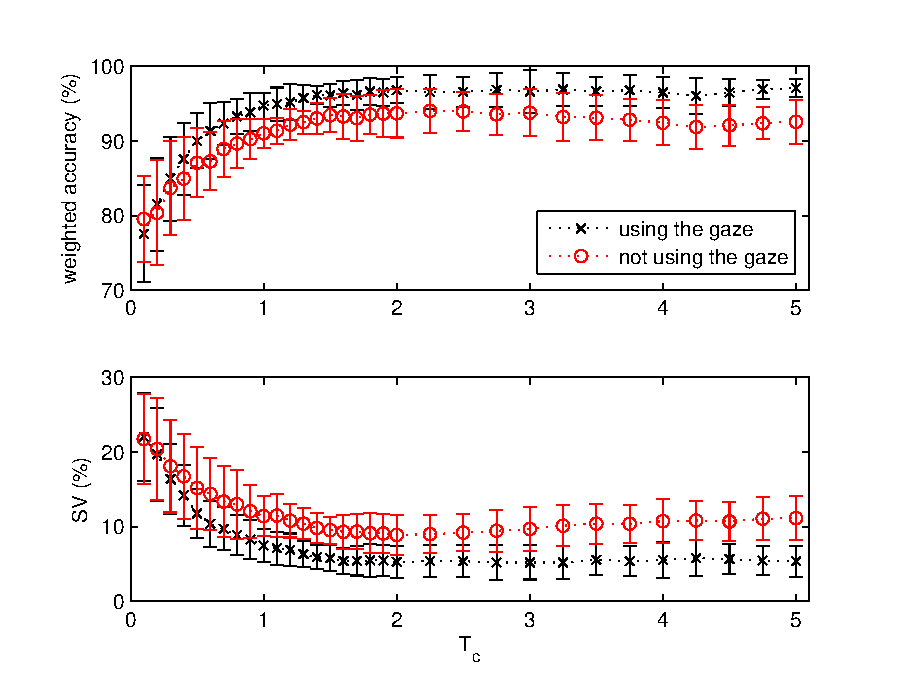
\includegraphics[width=\linewidth]{figs/comparison.eps}
    \caption{Comparison between not using the gaze (red curve) and
    using the gaze (black one) as $T_c$ increases. Top panel: weighted
    accuracy. Bottom panel: size of the models, expressed as the
    fraction of Support Vectors. Dots are the mean values over all
    subjects, whereas the errorbars denote $\pm$ one standard deviation.}
    \label{fig:comparison}
\end{figure}

First of all, the effect predicted in the previous Section is present:
both the accuracy and size of the models become better as $T_c$ is
increased, and reach a maximum around $T_c=2$ seconds; then they
remain essentially constant. Secondly, notice that the use of the gaze
uniformly and consistently improves both the accuracy of the models
and their size, the black curve being systematically higher than the
red one, as far as the accuracy is concerned, and lower in the case of
the model size. For $T_c\geq 2$, there is little overlap among the
errorbars, indicating a stastically significant improvement. Thirdly,
it seems that such a value of $T_c$ is just about right for all
subjects, notwithstanding their differences; we then conclude that
$\tau(i)$ is essentially the same for all subjects. This could
dramatically reduce the setup time in a real setting.

For $T_c=2$ seconds, the accuracy is $96.79\% \pm 1.7\%$ using the
gaze, as opposed to $93.69\% \pm 3.24\%$ when not using it; the model
size is $5.27\% \pm 2.12\%$ as opposed to $8.88\% \pm 2.73\%$. The
mean values are better, and the standard deviations are smaller when
using the gaze, denoting better performance and higher robustness with
respect to the diversity of the subjects.

Let us then turn to the experiment with the gaze, and analyse the
performance in deeper detail for the single subjects. Figure
\ref{fig:subjects} shows the same results as the black curves of Figure
\ref{fig:comparison}, but for each subject.

\begin{figure*}[!ht]
  \centering
    \begin{tabular}{cc}
      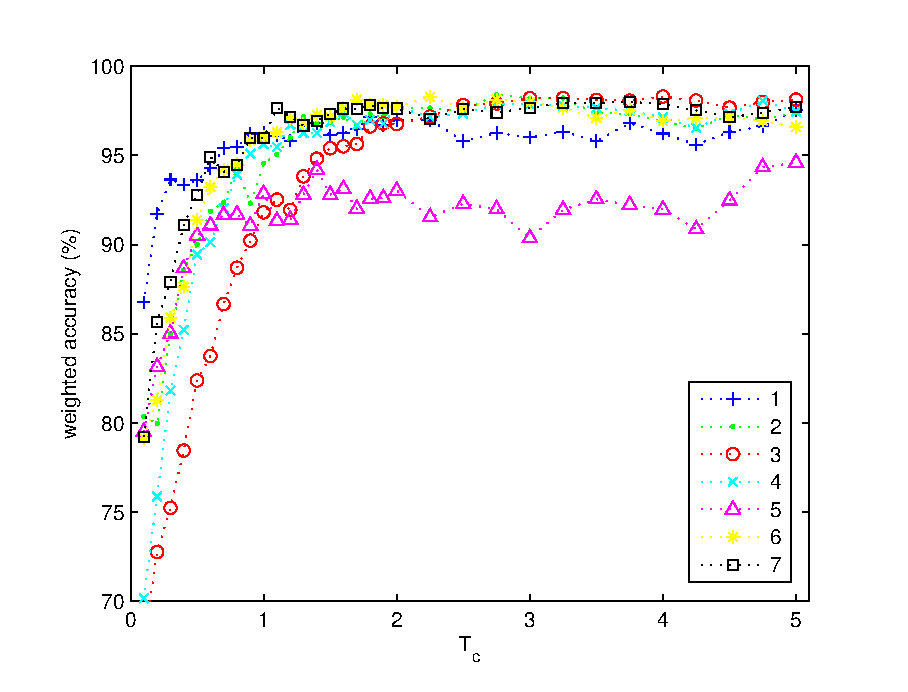
\includegraphics[width=0.45\textwidth]{figs/subjects_acc.eps} &
      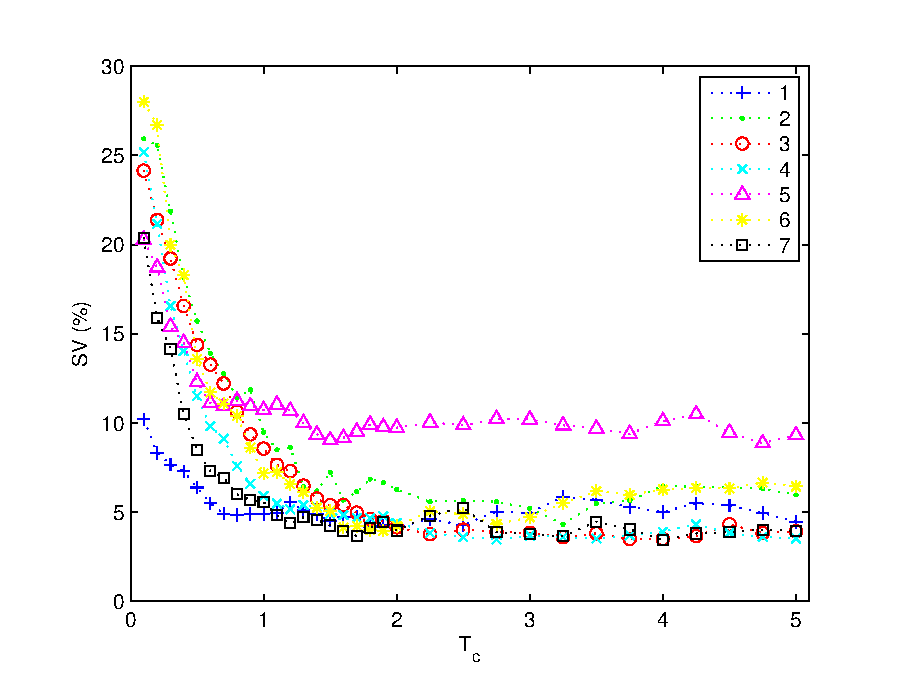
\includegraphics[width=0.45\textwidth]{figs/subjects_size.eps} \\
      $(a)$ & $(b)$ \\
    \end{tabular}
    \caption{Accuracy $(a)$ and size $(b)$ of the models for each single subject,
    using the gaze.}
    \label{fig:subjects}
\end{figure*}

Consider the Figure, panel $(a)$: it is apparent that the worst
subject is number $5$, a 73-years old woman who has undergone in the
past a cataract surgical operation. It is not surprising that this is
the hardest subject; still, for $T_c=2$, the model has a remarkable
accuracy of $93.03\%$. All other subjects reach an accuracy of
$96.75\%$ and more for the same value of $T_c$. Analogous
considerations apply as far as the model size is concerned (panel $(b)$
of the same Figure). It is interesting to note that, even for such a
hard subject as subject $5$, the use of the gaze signal greatly
improves the accuracy of the model (see Figure \ref{fig:mama}).

\begin{figure}[!ht]
  \centering
    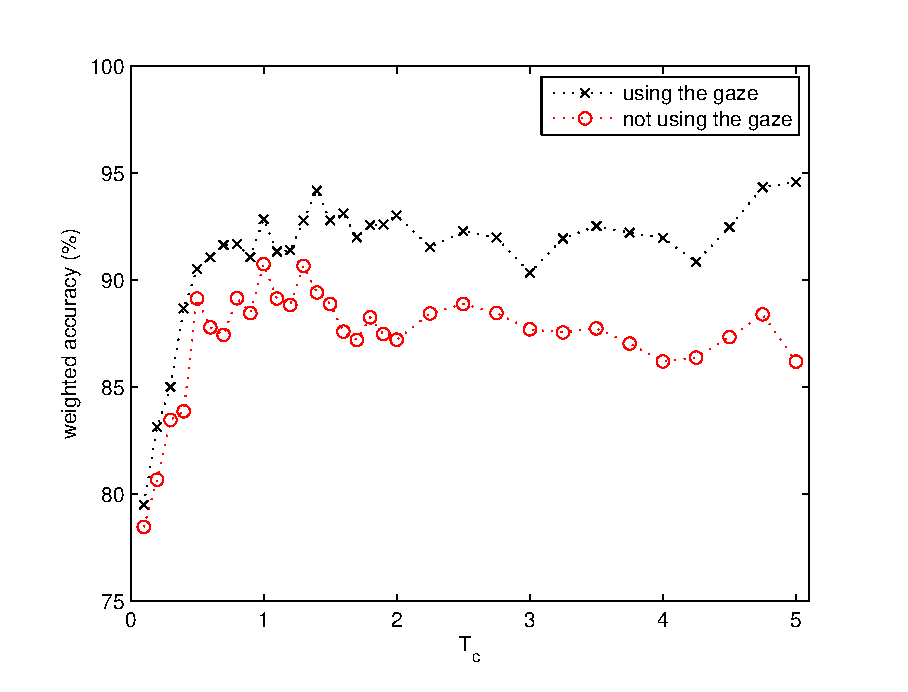
\includegraphics[width=\linewidth]{figs/mama.eps}
    \caption{Comparison between not using the gaze (red curve) and
    using the gaze (black one) as $T_c$ increases, for subject $5$.}
    \label{fig:mama}
\end{figure}

\subsection{Cross-subject analysis}

One further interesting point is: how well can these models be
transferred across subjects? In other words: are models trained on a
certain subject $i$ good for predicting the intention of another
subject $j$? Does gaze improve the situation? And, what are the
``hardest'' subjects to be modelled? In order to answer these
questions we have tested each model for $T_c=2$ on data gathered from
all subjects, both when using and not using the gaze. Figure
\ref{fig:cross} shows the results as cross-accuracy matrices: in each
matrix $A$, the entry $A_{ij}$ represents in colour the accuracy
attained by the model trained on subject $i$ when tested on data
gathered from subject $j$.

\begin{figure*}[!ht]
  \centering
    \begin{tabular}{cc}
      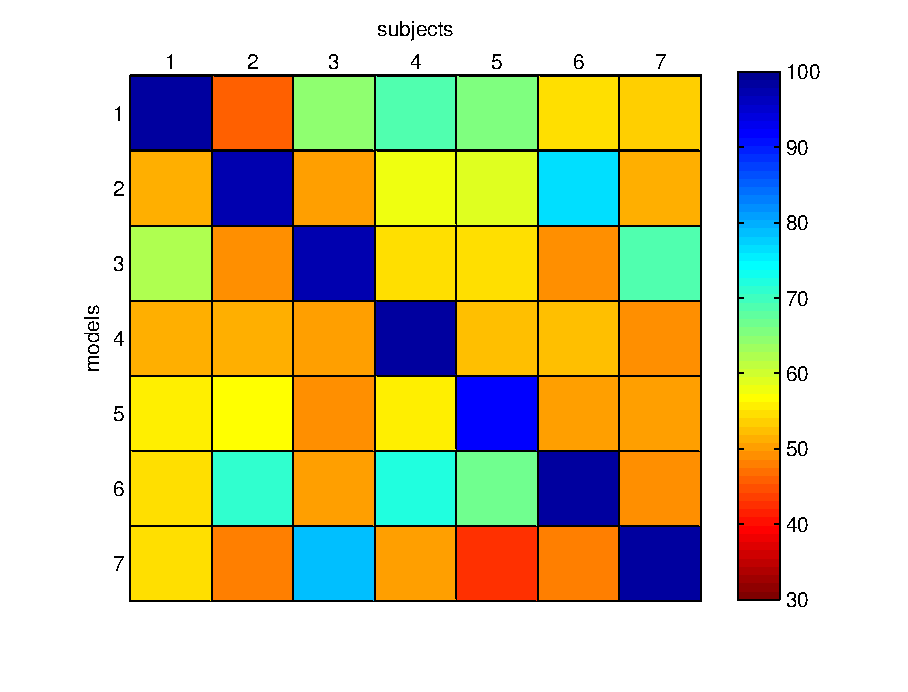
\includegraphics[width=0.45\textwidth]{figs/cross_nogaze.eps} &
      \includegraphics[width=0.45\textwidth]{figs/cross_gaze.eps} \\
    \end{tabular}
    \caption{Cross-subject accuracy, not using the gaze (left panel,
    accuracy $55.97\% \pm 8.6\%$) and using the gaze (right panel,
    accuracy $61.32\% \pm 11.77\%$).}
    \label{fig:cross}
\end{figure*}

As is apparent, using the gaze improves the situation: the overall
accuracy (not considering the diagonal elements of the matrices, of
course) is $55.97\% \pm 8.6\%$ when not using the gaze, as opposed to
$61.32\% \pm 11.77\%$ when using the gaze. In general these figures
are not very good, meaning that there is little chance that models can
be transferred across subjects, even when using the gaze.

Let us now restrict to the experiment with the gaze (right panel of the
Figure). The worst model (row of the matrix) is, unsurprisingly,
obtained from subject number $5$, with an accuracy of $49.31\% \pm
2.8\%$; as well, the hardest subject (column of the matrix) is again
number $5$, with an accuracy of $56.70\% \pm 9.09\%$. Subject $5$ has
to be treated on her own. But as well, again, let us remark that the
two best models, obtained from subjects $2$ ($73.99\% \pm 7.89\%$) and
$6$ ($70.32\% \pm 6.61\%$) still show a poor trasnferability as well
--- compare these figures with those of the previous Subsection.

%%%%%%%%%%%%%%%%%%%%%%%%%%%%%%%%%%%%%%%%%%%%%%%%%%%%%%%%%%%%%%%%%%%%%%%%%%%%%%%%
\section{Discussion and Conclusions}

\label{sec:concl}

In this paper we have shown that good artificial internal models of
when to grasp can be obtained by applying Support Vector Machines to
data gathered from diverse human subjects, engaged in a simple
grasping experiment in a teleoperation scenario. The data consisted of
the hand velocity and the gaze signal, which was proved to be crucial
in improving the performance of the models, both in terms of accuracy
and size.

Interestingly, about the same characteristic time value for $T_c$ can
be found for all subjects, the best models being found for $T_c=2$
seconds. The system greatly benefits from the use of gaze tracking,
also in case the subjects are visually impaired (subject $5$).

The models obtained for each subject are $(a)$ highly accurate, giving
the correct guess in $96.79\% \pm 1.7\%$ of the cases; and $(b)$
small, and therefore fast and usable in an on-line environment, the
percentage of support vectors for each model being $5.27\% \pm
2.12\%$. Analogous figures when the gaze is not used are sensibly
worse. The accuracy and size of the best models for each subject are
remarkable, meaning that the system is also very flexible and
unhindered by the subjects' diverse abilities and visual impairments.

Cross-subject transferability of models is, on the other hand, so far
unfeasible, the figures showing that models trained on a subject
cannot in general obtain good accuracy values when applied to data
gathered from different subjects. But this does not seem of any
hindrance to the approach, since the models can be trained, in the
worst case, using $3.5$ minutes of user data. Independent training for
each subject can then be performed with a reasonable effort.

%%%%%%%%%%%%%%%%%%%%%%%%%%%%%%%%%%%%%%%%%%%%%%%%%%%%%%%%%%%%%%%%%%%%%%%%%%%%%%%%

\bibliography{paper}

\end{document}
